\documentclass[conference]{IEEEtran}

\usepackage{graphicx}
\usepackage{subfigure}
\usepackage{amsmath}
\usepackage{amssymb} 
\usepackage{array}
\usepackage{booktabs}
\usepackage{multirow}
\usepackage{array,booktabs,tabularx}
\usepackage{blindtext}
\usepackage{color}
\usepackage[colorlinks=true, linkcolor=blue, citecolor=blue, urlcolor=blue]{hyperref}
\usepackage[all]{hypcap}
\usepackage{float}
\usepackage{subcaption}

\usepackage{etoolbox}
\makeatletter
\patchcmd{\@eqnnum}{\hb@xt@.01\p@}{\hypertarget{equation.\theequation}{}}{}{}
\makeatother

\def\BibTeX{{\rm B\kern-.05em{\sc i\kern-.025em b}\kern-.08em
    T\kern-.1667em\lower.7ex\hbox{E}\kern-.125emX}}
\usepackage{mwe}
\usepackage{fancyhdr}
\fancypagestyle{firststyle}
{
	\fancyhf[C]{\fontsize{8}{10} \selectfont \textit{} }
	\fancyfoot[C]{}
}

\newcolumntype{C}[1]{>{\centering\arraybackslash}m{#1}}
%\hyphenation{ }

\begin{document}

% Do not put math or special symbols in the title.
\title{Determinación de parametros del generador síncrono usando pruebas de simulación de rechazo de carga}


\author{
\IEEEauthorblockN{José de Jesús Reyes Ramírez\IEEEauthorrefmark{1},
Yosniel\IEEEauthorrefmark{2},
Luis\IEEEauthorrefmark{3},
Gary\IEEEauthorrefmark{4},
Aylem\IEEEauthorrefmark{5}}
\IEEEauthorblockA{\textit{Universidad de Guadalajara, CUCEI} \\
\textit{Maestría en Ciencias en Ingeniería Eléctrica} \\
Guadalajara, Jalisco, México \\
\IEEEauthorrefmark{1}jose.reyes0963@alumnos.udg.mx,
\IEEEauthorrefmark{2}@alumnos.udg.mx,
\IEEEauthorrefmark{3}@alumnos.udg.mx,
\IEEEauthorrefmark{4}a@alumnos.udg.mx,
\IEEEauthorrefmark{5}@alumnos.udg.mx}
}


\maketitle

\thispagestyle{firststyle}
\renewcommand{\headrulewidth}{0in}
\pagestyle{empty}

\pagestyle{fancy}
\chead{\fontsize{8}{10} \selectfont \textit{} }
\pagenumbering{gobble}

\begin{abstract}
	En el presente se muestra como obtener los parámetros estándar del generador síncrono a partir simulaciones de pruebas de rechazo de carga en Matlab/Simulink.
\end{abstract}

\section{Introducción}
El generador síncrono es \dots

Los parámetros fundamentales del generador síncrono son: $r_s$, $r_{fd}$, $r_{kd}$, $r_{kq1}$, $r_{kq2}$, $x_{Ls}$, $x_{1fd}$, $x_{lkd}$, $x_{lkq1}$, $x_{lkq2}$, $x_{md}$ y $x_{mq}$. Los cuales se calculan usando relaciones matemáticas.

Los parámetros estándar del generador síncrono son las reactancias síncronas, las reactancias síncronas transitorias, las reactancias síncronas subtransitorias, las constantes de tiempo transitorias y subtransitorias en circuito abierto y las constantes de tiempo transitorias y subtransitorias en cortocircuito; es decir, $x_d$, $x_q$, $x^{'}_d$, $x^{'}_q$, $x^{''}_d$, $x^{''}_q$, $T^{'}_{do}$, $T^{'}_{qo}$, $T^{''}_{do}$, $T^{''}_{qo}$, $T^{'}_{d}$, $T^{'}_{q}$, $T^{''}_{d}$, $T^{''}_{q}$.

La identificación de sus parámetros de estado permanente y transitorio es muy importante para el análisis de estabilidad, esto debido a \dots

Existen principalmente 2 pruebas para la determinación de parámetros de un generador síncrono, los cuales han obtenido importancia debido al bajo nivel de riesgo y a su facilidad, los cuales son el método de respuesta en frecuencia y el método de rechazo de carga.

La prueba de respuesta en frecuencia consiste en aplicar una corriente con frecuencias que varíen en el rango de 0.001 Hz a 1 kHz, la cual es aproximadamente del \% de la corriente nominal. Usando los datos de la respuesta en frecuencia obtenidos de la prueba se determinan parámetros estándar de la máquina, es decir, las constantes de tiempo y las reactancias sincronas, transitorias y subtransitorias de los ejes directo y en cuadratura.

El método de rechazo de carga consiste en realizar pruebaas de rechazo de carga en dos puntos operativos, donde las componentes de corriente sólo existan en el eje de interés. La prueba en el eje directo se realiza subexcitando el generador, por lo que debe estar consumiendo potencia reactiva de la red y la potencia activa debe ser despreciable, debido a la excitación insuficiente. Lo cual garantiza la obtención de parámetros no saturados y evita sobretensiones indeseadas durante la prueba. Los datos que permite obtener la prueba en el eje directo son $x_d$, $x^{'}_d$, $x^{''}_d$, $T^{'}_{do}$ y $T^{''}_{do}$.

La prueba en el eje de cuadratura se realiza encontrando un punto de carga en el cual el valor absoluto del ángulo del factor de potencia sea igual al ángulo de potencia, esto con el generador subexcitado.


\section{Pruebas de Rechazo de Carga para Determinación de Parámetros de Generadores Síncronos} 

Las pruebas de rechazo de carga constituyen una metodología estandarizada según las normas IEEE 115
para la determinación experimental de los parámetros operativos de generadores síncronos. Estas pruebas
se realizan mediante la desconexión brusca del generador del sistema de potencia, manteniendo constante
la tensión de campo y registrando la respuesta transitoria de las variables eléctricas.

\subsection{Prueba de rechazo de carga en el eje directo $-d-$}

La prueba de rechazo de carga en el eje $-d-$ se ejecuta con el generador entregando potencia activa nula y potencia reactiva máxima,
condiciones bajo las cuales la corriente de armadura se alinea exclusivamente con el eje directo.
Durante el rechazo de carga, se registra el decaimiento transitorio de la tensión terminal, cuyo análisis
permite determinar las reactancias síncrona, transitoria y subtransitoria del eje directo ($x_d, x^{'}_d, x^{''}_d$) así como las constantes
de tiempo en circuito abierto ($T^{'}_{qo}$, $T^{''}_{do}$)

\subsection{Prueba de rechazo de carga en el eje en cuadratura $-q-$}

Para esta prueba, se ajusta la operación del generador de modo que el ángulo de potencia coincida con el ángulo del factor de potencia,
logrando que la corriente de armadura posea únicamente componente en cuadratura. El análisis del transitorio de tensión resultante del
rechazo de carga permite calcular la reactancia síncrona y subtransitoria del eje $q$ ($x_q, x^{''}_q$)

\subsection{Prueba de rechazo de carga en el eje arbitrario}

Esta prueba representa la metodología más comprehensiva, ya que se realiza con el generador operando en condiciones de carga arbitrarias,
con componentes de corriente tanto en el eje directo como en cuadratura. El procesamiento de la respuesta transitoria, particularmente de
la componente en cuadratura de la tensión y corriente, permite determinar el conjunto completo de parámetros del eje q 
($x_q, x^{'}_q, x^{''}_q, T^{'}_{qo}$, $T^{''}_{do}$)

\section{Simulación y resultados obtenidos}
Para determinar los parámetros del generador se utilizó como base el esquema mostrado en la Fig. \ref{fig:Modelo_Simulink}

\begin{figure}[H]
    \centering
    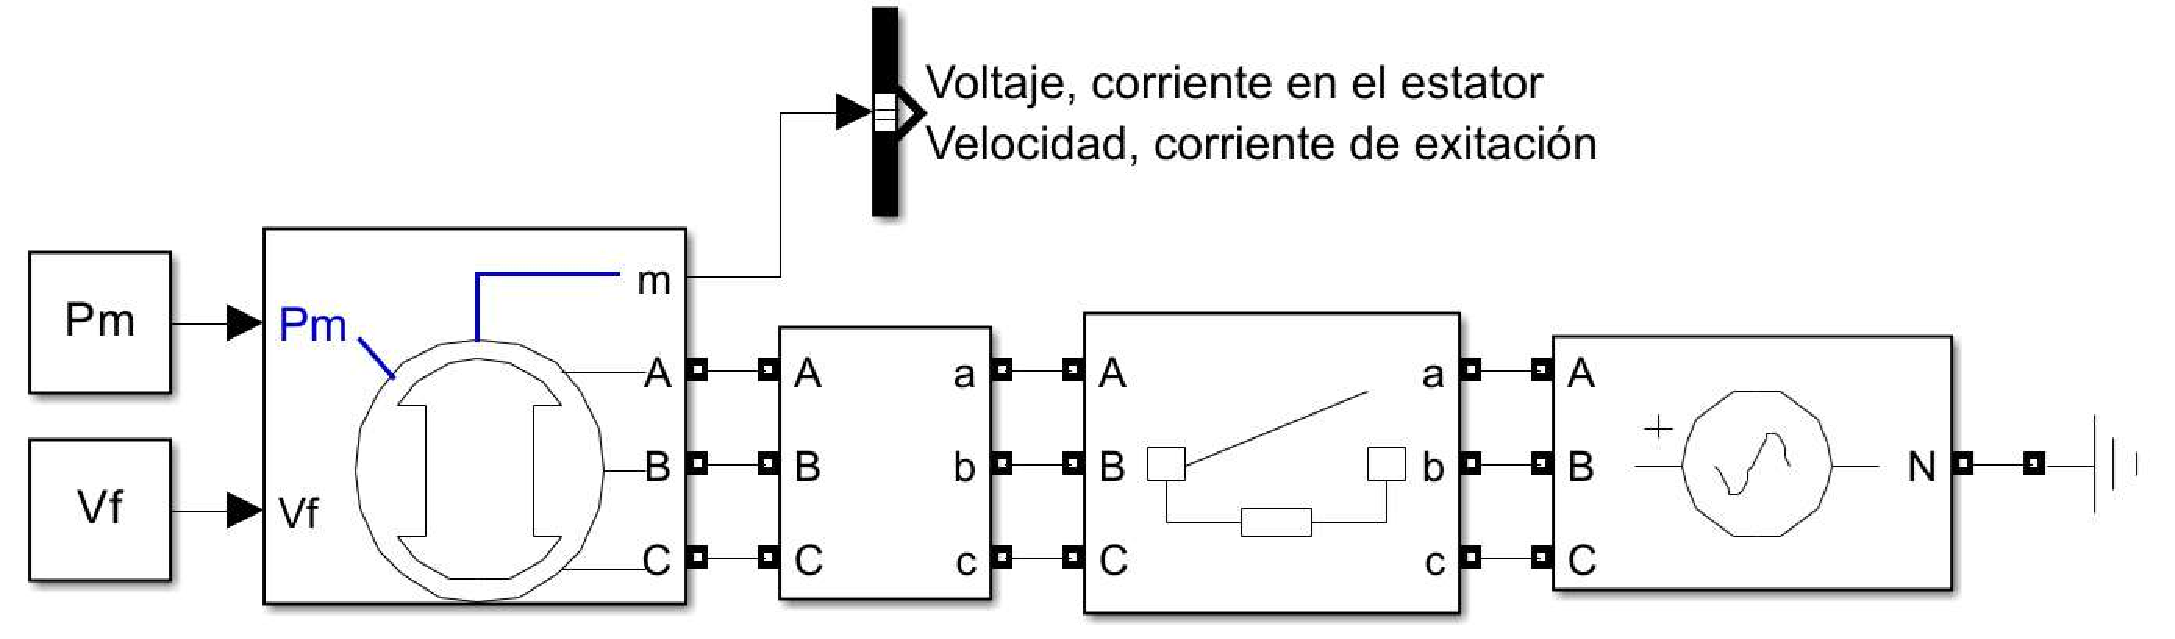
\includegraphics[width=\linewidth]{Fig/Modelo_Simulink.pdf}
    \caption{Modelo base implementado en Simulink}
    \label{fig:Modelo_Simulink}
\end{figure}

\subsection{Prueba de rechazo de carga en el eje $-d-$}

Para esta prueba se verifica antes del rechazo de carga que $P_0=0\text{ pu}$, $Q_0=0.1239\text{ pu}$ (capacitive load),
$V_{t_0}=1\text{ pu}$, $i_{t_0}=0.1239\text{ pu}$ y $v_f=0.87\text{ pu}$.

Para el rechazo de carga en $t=25\text{ s}$, se obtiene el comportamiento para la tensión
en los terminales de generador ($v_t$) mostrados en la Fig. \ref{fig:fig1}.

\begin{figure}[H]
    \centering
    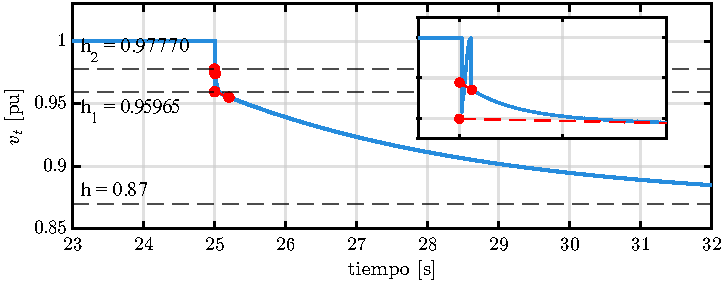
\includegraphics[width=\linewidth]{Fig/fig1.pdf}
    \caption{Voltaje en terminales de la máquina durante el rechazo de carga}
    \label{fig:fig1}
\end{figure}

Para calcular los valores de reactancias se obtiene las intersecciones en las tendencias del
voltaje terminal con el eje del voltaje terminal en el momento que ocurre el rechazo de carga
como muestra la Fig. \ref{fig:fig1}. Utilizando estos valores se calculan las reactancias como
se muestra a continuación, donde $A=1-h_2$, $B=1-h_1$ y $C=1-h$:

\begin{gather*}
x_d = \frac{C}{i_{t_0}} = \frac{1 - 0.87}{0.1239} = 1.0492\text{ pu} \\
x'_{d} = \frac{B}{i_{t_0}} = \frac{1 - 0.95965}{0.1239} = 0.3257\text{ pu}\\
x''_{d} = \frac{A}{i_{t_0}} = \frac{1 - 0.97770}{0.1239} = 0.18\text{ pu}\\
\end{gather*}

Para determinar las constantes de tiempo de circuito abierto se utiliza la curva de corriente de campo
obtenida durante el rechazo de carga mostrado en la Fig. \ref{fig:fig2}

\begin{figure}[H]
    \centering
    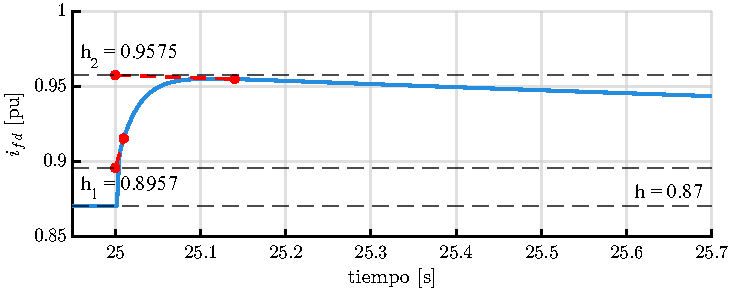
\includegraphics[width=\linewidth]{Fig/fig2.pdf}
    \caption{Corriente de exitación durante el rechazo de carga}
    \label{fig:fig2}
\end{figure}

\subsection{Prueba de rechazo de carga en el eje $-q-$}

Para esta prueba se verifica antes del rechazo de carga que $P_0 = 0.6249\text{ pu}$, $Q_0 = 0.3054\text{ pu}$ (carga
capacitiva), $V_{t_0} = 1\text{ pu}$, $i_{t_0} = i_{q_0} = 0.6665\text{ pu}$, $v_f = 0.87\text{ pu}$, $\delta_0 = \varphi_0 = 26.05^{\circ}$.


Durante esta prueba se obtiene el comportamiento para $\omega_r$ y $V_t$ mostrados en las Fig. \ref{fig:subfigs} respectivamente.

\begin{figure}[H]
    \centering
    \begin{subfigure}
        \centering
        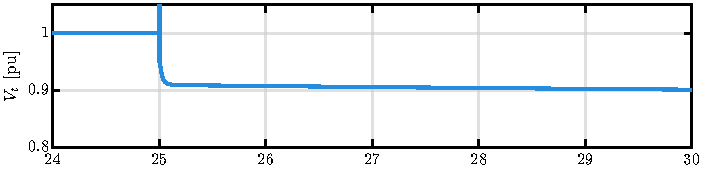
\includegraphics[width=\linewidth]{Fig/fig3.pdf}
        %\caption{figura 1}
        \label{fig:fig3}
    \end{subfigure}
    \hfill
    \begin{subfigure}
        \centering
        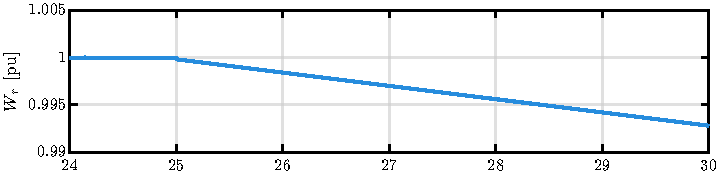
\includegraphics[width=\linewidth]{Fig/fig4.pdf}
        %\caption{figura 2}
        \label{fig:fig4}
    \end{subfigure}
    \hfill
    \begin{subfigure}
        \centering
        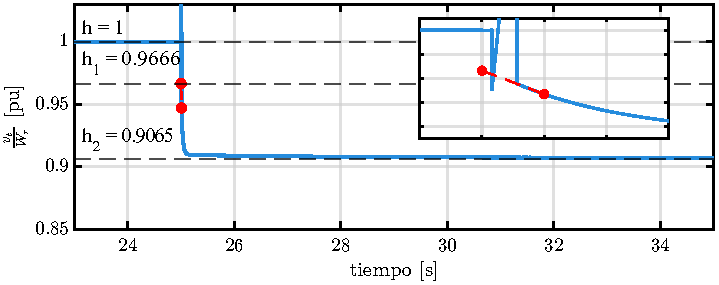
\includegraphics[width=\linewidth]{Fig/fig5.pdf}
        
        \label{fig:fig5}
    \end{subfigure}
    \caption{Comportamiento de $V_t$ y $\omega_r$ durante la prueba de rechazo de carga en el eje $-q-$}
    \label{fig:subfigs}
\end{figure}

Para determinar los parámetros de $x'_q$ y $x''_q$ se procede como se muestra a continuación, donde
$A=1$, $B=h_1=0.9666\text{ pu}$ y $C=h_2=0.9065\text{ pu}$.

\begin{gather*}
x_q = \frac{\sqrt{A^2-C^2}}{i_{q_0}} = \frac{\sqrt{1^2 - 0.9065^2}}{0.6665} = 0.6334\text{ pu} \\
x''_q = \frac{\sqrt{A^2-C^2}-\sqrt{A^2-B^2}}{i_{q_0}}=\cdots\\
\cdots= \frac{\sqrt{1^2-0.9065^2}-\sqrt{1^2-0.9666^2}}{0.6665} = 0.2489\text{ pu}\\
\end{gather*}

\subsection{Prueba de rechazo de carga en el eje arbitrario}.

Las cantidades electricas en el instante antesa que se realiza el rechazo de carga son: $P_0 = 0.8437pu$, $Q_0 = 0.5222pu$, $V_t = 1.0003pu$, $i_{t0} = 0.5729pu$, $v_f = 1.7688pu$, $\delta_0 = 20.8946$.
Usando las expresiones dadas em ***, en los datos de las Fig.\ref{fig:subfigs1}, los parametros $x_q$ y $x''_q$ se pueden calcular de la siguiente manera:

\begin{gather}
    x_q = \frac{(V_t\sin(\delta))_0}{i_{qo}}\\
    x''_q = x_q\frac{h}{i_{qo}}
\end{gather}

\begin{figure}[ht]
    \centering
    \begin{subfigure}
        \centering
        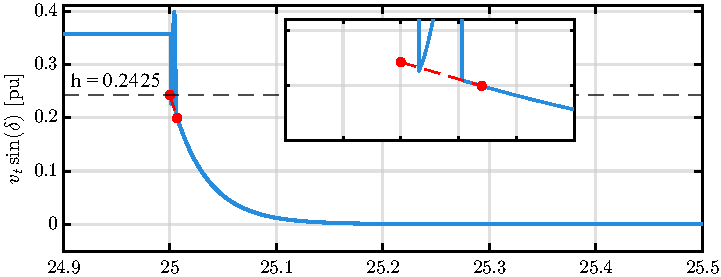
\includegraphics[width=\linewidth]{Fig/fig6.pdf}
        %\caption{figura 1}
        \label{fig:fig6}
    \end{subfigure}
    \hfill
    \begin{subfigure}
        \centering
        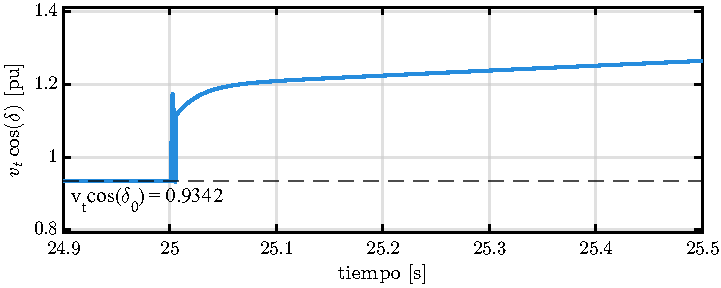
\includegraphics[width=\linewidth]{Fig/fig7.pdf}
        %\caption{figura 2}
        \label{fig:fig7}
    \end{subfigure}
    \hfill
    \begin{subfigure}
        \centering
        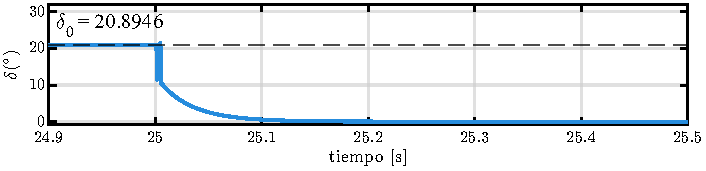
\includegraphics[width=\linewidth]{Fig/fig8.pdf}    
        \label{fig:fig8}
    \end{subfigure}
    \caption{Comportamiento de $V_t$ y $\delta_0$ durante la prueba de rechazo de carga en el eje arbitrario}
    \label{fig:subfigs1}
\end{figure}

\subsection{Resultados generales}


\setlength{\extrarowheight}{2pt} % eleva todas las filas
\begin{table}[ht]
\centering
\caption{Parametros en p.u.}
\setlength{\tabcolsep}{6pt}
\begin{tabular}{C{1cm} C{1cm} C{1cm} C{1cm} C{1cm} C{1.25cm}}
\toprule
\textbf{Parametro} &
\textbf{Rechazo de carga en el eje directo} &
\textbf{Rechazo de carga en el eje directo} &
\textbf{Rechazo de carga en eje arbitrario} &
\textbf{Calculados} & 
\textbf{Valores de diseño} \\
%\cmidrule(lr){5-6}
%\multicolumn{1}{c}{} &
%\multicolumn{1}{c}{\textbf{Load Rejection}} &
%\multicolumn{1}{c}{\textbf{Load Rejection}} &
%\multicolumn{1}{c}{\textbf{Load Rejection}} &
%\textbf{Calculated} & \textbf{Design Values} \\
\hline
\midrule
$T'_{do}$ & 3.8955 & --     & --     & --     & 3.7724 \\
$T''_{do}$ & 0.0245 & --     & --     & --     & 0.0238 \\
$T''_{qo}$ & --     & --     & 0.0333 & --     & 0.0334 \\
$x_d$ & 1.0492 & --     & --     & --     & 1.0495 \\
$x_q$ & --     & 0.6334 & 0.6224 & --     & 0.6313 \\
$x'_d$ & 0.3257 & --     & --     & --     & 0.3320 \\
$x''_d$ & 0.18 & --     & --     & --     & 0.1963 \\
$x''_q$ & --     & 0.2489 & 0.1991 & --     & 0.2496 \\
$T'_d$ & --     & --     & --     & 1.2093 & 1.1939 \\
$T''_d$ & --     & --     & --     & 0.0135 & 0.0140 \\
$T''_q$ & --     & --     & --     & 0.0131 & 0.0132 \\
\bottomrule
\end{tabular}
\end{table}


\section{Conclusiones}
Se concluye que 

\begin{thebibliography}{plain}
\bibitem{b1} M. H. Rashid, Power Electronics: Devices, Circuits \& Applications, Pearson Education, 2013.
\bibitem{b2} Mohan N., Undeland T. M., Robbins W. P. (2002) Power Electronics: Converters, Applications, and Design, Wiley.
\end{thebibliography}

\end{document}